\chapter{ExxonMobil Model}
\label{ch:exxonmobilmodel}

\section{Introduction}
The model employs a coupled axial-torsional system, meticulously considering interactions among various elements, such as drill pipes, HWDP, and collars. Through a lumped-parameter study, the model enables thorough investigations into the impacts of different operational conditions on drill string behavior. Additionally, it integrates friction models to accurately represent the axial and tangential forces acting along the drill string, as well as the bit-rock interaction model (IADC/SPE-199678) to explain the cause of stick-slip. This model features 4 degrees of freedom per node, encompassing axial displacement, axial velocity, angular displacement, and angular velocity.The governing equations of both torsional and axial motion are solved by finite element method (FEM). The validation of the model is achieved by comparing simulation results with field data from rotational startups, off-bottom rotations, and post-connection operations. 

In the axial direction, the displacement is one-dimensional, while in the rotational direction, equations are coupled using the Striebeck friction model. This model takes into account the resultant velocity to accurately compute friction forces. Notably, the model incorporates well trajectory and buoyancy effects to ensure precise calculation of resultant friction forces. Furthermore, it uniformly applies drag due to mud throughout the system. The model's ability to simulate Mud-motor and Heave compensator dynamics enhances its versatility. The bit-rock interaction model is based on depth-of-cut, while simultaneously tracking the revolution of bit-depth relative to hole-depth. This feature contributes to a more realistic representation of the drilling process.

Following features are described for bit-rock and friction models below:
\begin{bulletedlist}
    \item Bit-rock interaction model is coupled with bit's displacement and angular displacement.
    \item Drilling mode gets activated when the DOC and angular displacement are higher than 0. (Clockwise rotation) 
    \item Friction model is coupled i.e, resultant reaction force from axial and tangential direction is taken into account.
    \item No movement until the resultant reaction force reaches static limit.
    \item Coulomb friction model is implemented when the drill string is in motion.
    \item The friction state is tracked for each element.
\end{bulletedlist}

The Python-based source code is designed with a modular approach, wherein most functions are distributed across separate Python files, easily accessible by importing them. The code's operational instructions and guidelines are included in the provided manual, offering users comprehensive guidance on running the code effectively.

\section{Features}
\subsection{Top-drive Model}

The model utilizes the axial and rotational velocity magnitudes of the top-drive as input and primarily computes the area under the velocity curve. It then provides outputs for axial and rotational top-drive velocities, as well as the corresponding displacements and rotations of the top-drive.

Torque on top-drive can be derived as:
\begin{equation}\label{TorqueEQ}
  \tau_{top\_drive} = k_{t1} \times \theta_{top\_drive}
\end{equation}

where 
$\tau_{top\_drive}$ is top-drive torque, $k_{t1}$ is torsional stiffness of first drill-string element, and $\theta_{top\_drive}$ is top-drive rotation.

Furthermore, the model incorporates an additional parameter known as "Heave." If the runtime surpasses the Heave delay, additional computations are conducted to determine Heave displacement and Rate of Penetration (ROP). These calculated values are subsequently added to the original top-drive ROP and displacement data. The Heave ROP and displacement calculations are represented by the following equations:

\begin{equation}\label{Z_heave}
  Z_{heave} = x \cdot \sin(\omega \cdot (t - t_{heave\_delay}))
\end{equation}

\begin{equation}\label{ROP_heave}
  ROP_{heave} = x \cdot \omega \cdot \cos(\omega \cdot (t - t_{heave\_delay}))
\end{equation}

where 
$Z_{heave}$ and $ROP_{heave}$ are Heave displacement and ROP, $x$ is Heave amplitude, $\omega$ is Heave angular velocity, $t$ is runtime and $t_{heave\_delay}$ is Heave delay time.
 
\subsection{Bit-rock Interaction Model}

The laws governing the bit-rock interface in drilling operations primarily rely on the relationships between Weight on bit, torque on bit, rate of penetration, and angular velocity. These interdependent variables play a crucial role in achieving efficient drilling while also influencing the emergence of drilling dysfunctions within the system. The forces and torque exerted on the bit are directly influenced by the instantaneous changes in axial and angular velocities.

The interaction between PDC bits and the rock formation encompasses a combination of cutting and frictional contact, as identified by (Detournay and Defourny in 1992). Weight on bit and torque on bit are further decomposed into cutting and frictional components, which are contingent upon the strength of the rock formation being drilled.

\begin{equation}\label{WOB}
  WOB_{bit} = (k_{WOB}\times DOC_{iteration}) + (c_{bit-axial\times \dot{Z}_{bit-ietration}})
\end{equation}

\begin{equation}\label{Torque}
  TQ_{bit} = k_{TQ}\times DOC_{iteration\; array}\times (\pm1)
\end{equation}

where $k_WOB$, $k_TQ$ is Weight on bit and Torque coefficient, $DOC_iteration$ is depth of cut per iteration, $C_{bit-axial}$ is axial drag coefficient of bit and $Z$ is bit displacement 

The cutting components exhibit a direct dependency on the depth of cut, representing the material removed during drilling, while the frictional components are considered to account for the dissipated energy in the drilling process. To enhance the assessment of frictional forces at the bit and along the length of the drill string, particularly in deviated wellbores, a consolidated friction model (IADC/SPE-199678) is implemented within the drilling simulator. 

\subsection{Friction Model}

Modeling friction forces along the drill string is a challenging task due to the system's nonlinear behavior and the continuous changes in velocity direction. The net frictional force is highly influenced by the sliding velocity, with the axial component contributing to drag force and the tangential component generating frictional torque within the system.
 
\begin{figure}
  \centering
  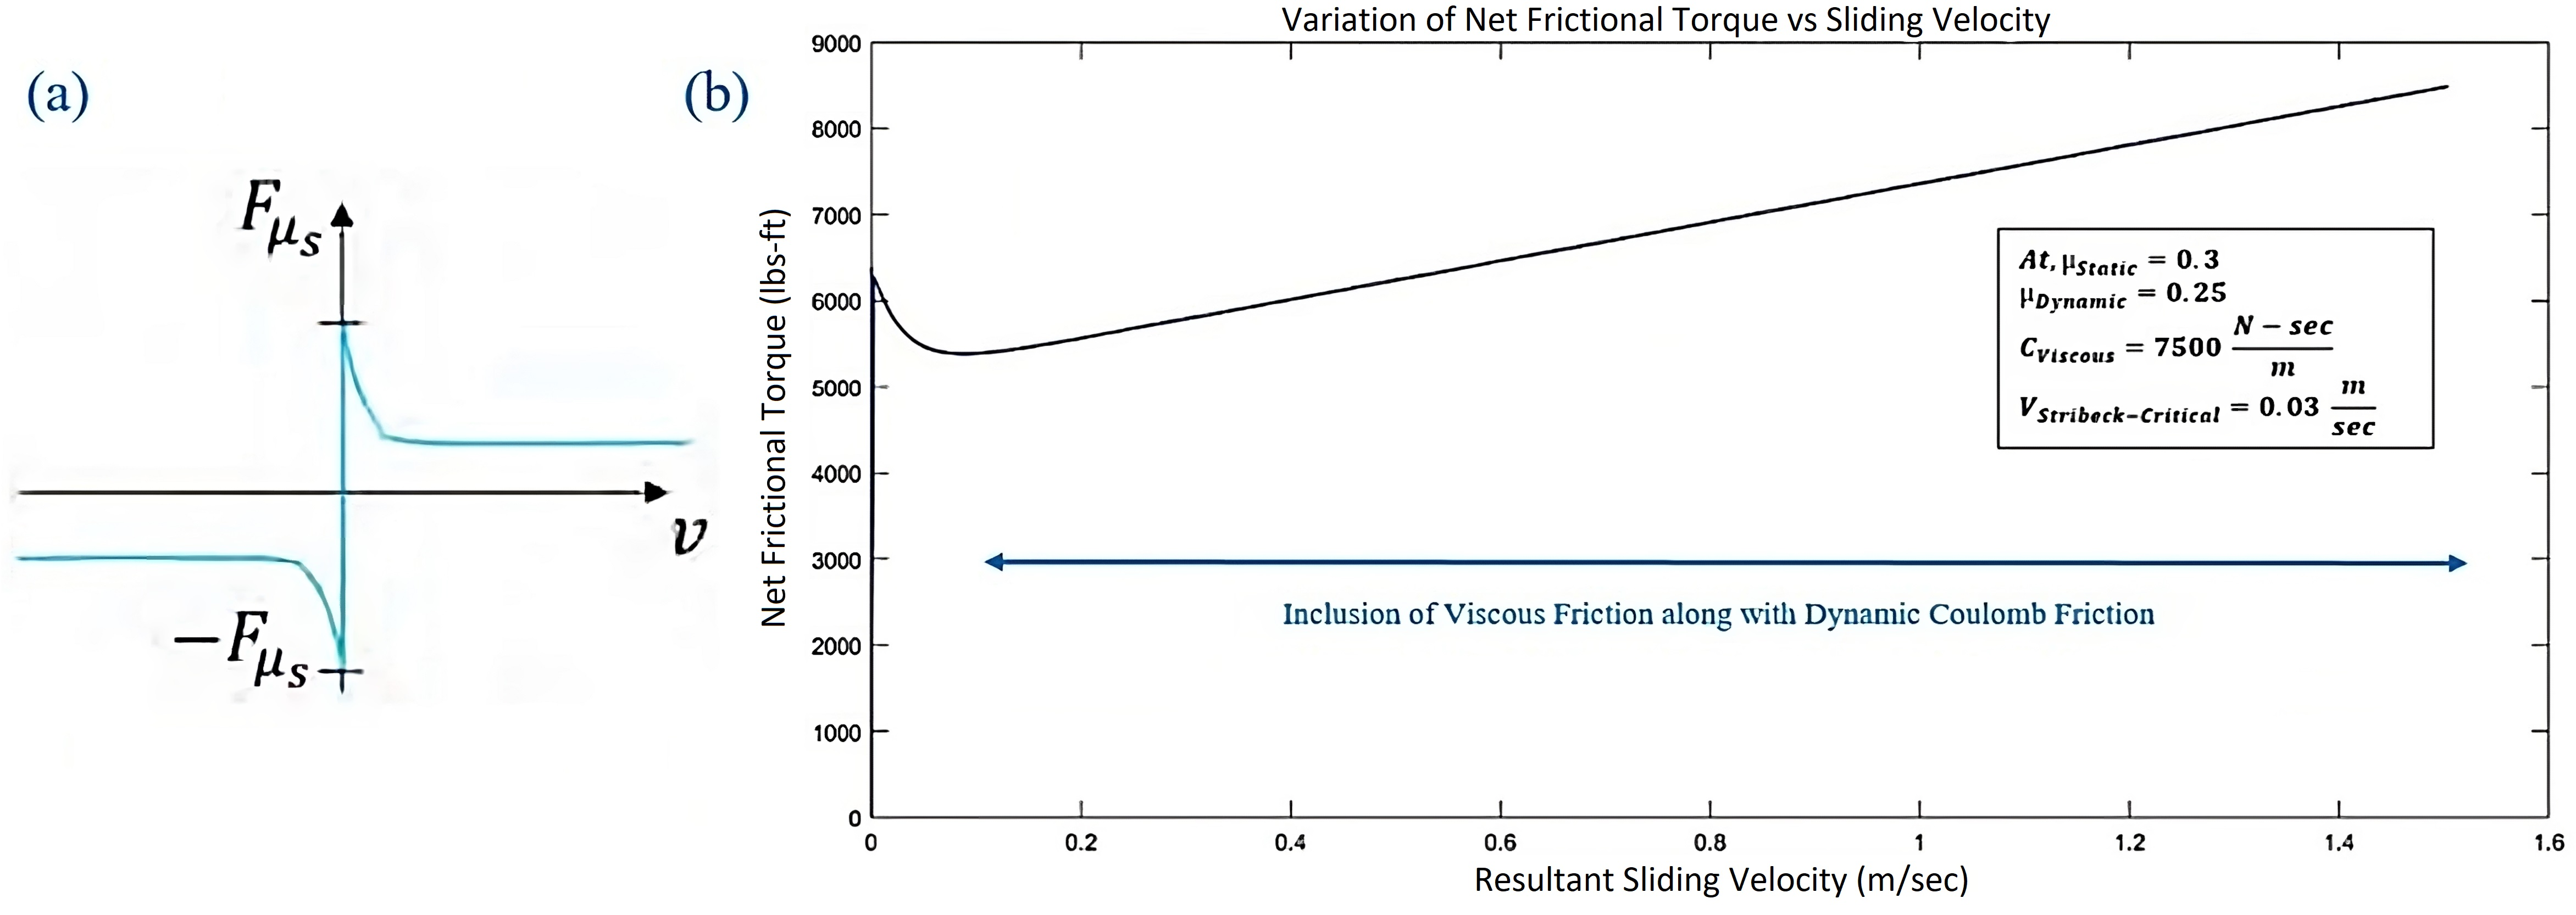
\includegraphics[width=6in]{Stribeck}
  \caption{Friction models: a) Without Viscous Friction , b) Coulomb + Viscous Friction}\label{Friction models}
\end{figure}

As the force of friction increases, it introduces a negative damping effect as the sliding velocity approaches zero. This negative damping effect can lead to stick-slip dysfunction, even when the bit is not in contact with the bottom of the well. In deviated wells, the axial velocity of the top drive and the drum's revolutions per minute do not instantaneously transfer to the bit. The elements of the drill string must overcome the static limits of friction to transfer energy to the next element. This lag in energy transfer is effectively described by the Stribeck curve, where the net frictional torque decreases as the sliding velocity increases.

\begin{equation}\label{dyanmic_force}
  F_{\mu\; k} = \mu_{k}\times F_{n} \times (Sign(V_{Sliding}))
\end{equation}

The dynamic friction force opposes the direction of axial motion, while static friction force $F_{\mu,s}$ acts in the opposite direction of the sum of all tangential forces when there is no sliding motion $V_{Sliding}=0$. The magnitude of the static friction force is equal to the sum of all tangential forces. This condition is valid when there is no sliding motion $V_{Sliding}=0$.

\begin{equation}\label{zero}
  F_{\mu,s} + \sum F_{Ext} = 0
\end{equation}

If, static friction calculated above is less than $\mu_{k}\times F_{n}$, where $\mu_{s} > \mu_{k}\times F_{n}$ then the surface is not sliding.

In order to avoid the discontinuities when $V_{iteration}$ tends to zero, Stribeck friction model is used. Following equation was proposed by Tustin 1947:

\begin{equation}\label{Stribeck velocity}
  F_{\mu,i} = F_{\mu_{k},i} + (F_{\mu_{s},i} - F_{\mu_{k},i})e^{-\dfrac{|\nu_{i}|}{\nu_{cs}}}
\end{equation} 

The model incorporates $F_{\mu,i}$ and $\nu_{CS}$ (Stribeck critical velocity) to consider the velocity weakening effect in the dynamics of the system. However, it should be noted that the model does not account for string Capstan effects.Furthermore, the order of the viscous damping constants is maintained consistently to ensure that the system remains in an ideal damp state, aligning with the field data. In the case of a multi-element string, the distribution of borehole dampers is considered by assigning damper values to each element based on the fraction of its mass contribution. For example, Collars are assigned 50\% of the damper value, HWDP is assigned 30\%, and drill-pipes are assigned 20\%. 

Below you will find the Friction model input parameters:

\begin{table}
  \centering
  \begin{tabular}{|c|}
    \hline
    % after \\: \hline or \cline{col1-col2} \cline{col3-col4} ...
    Equivalent diameter of pipe\\
    \hline
    Coulomb Friction Force \\
    \hline
    Coulomb Friction Force Axial Component \\
    \hline
    Coulomb Friction Force Tangential Component \\
    \hline
    Coulomb Friction Torque Tangential Component \\
    \hline
    Viscous Friction Force Axial Component \\
    \hline
    Viscous Friction Force Tangential Direction Component \\
    \hline
    Axial and Tangential components of Net Frictional Force and Torque \\
    \hline
  \end{tabular}
  \caption{Input parameters for Friction model}\label{Table_Friction_Input}
\end{table}

\section{Governing equations and solution}

The set of partial differential equations that describe the motion of the drill-string can be combined into a coupled axial-torsional system of second-order differential equations. 

\begin{equation}\label{Governing equations}
  \begin{cases}
   \begin{aligned}
     m_{i}\dfrac{\partial^{2}s_{i}}{\partial t^{2}} & = -k_{a,i}(s_{i}-s_{i-1}-l_{i}) + k_{a,j+1}(s_{i+1}-s_{i}-l_{i+1}) + \sum{F_{ext, i}} \\
     I_{i}l_{i}\dfrac{\partial^{2}\theta_{i}}{\partial t^{2}} & = -k_{t,i}(\theta_{i}-\theta_{i-1}-l_{i}) + k_{t,j+1}(\theta_{i}-\theta_{i+1}) + \sum{\tau_{ext,/ i}}
   \end{aligned}
  \end{cases}
\end{equation}

To convert these equation sets into vector form, we can represent the variables and their derivatives as vectors.

\begin{equation}\label{Vector_form}
  \begin{aligned}
  & \{M\} \ddot{\boldsymbol{Z}}+\left\{C_a\right\} \dot{\boldsymbol{Z}}+\left\{K_a\right\} \boldsymbol{Z}+\boldsymbol{f}_{\text {fric }}=\boldsymbol{F}_{\text {forcing }} \\
  & \{J\} \ddot{\boldsymbol{\theta}}+\left\{C_t\right\} \dot{\boldsymbol{\theta}}+\left\{K_t\right\} \boldsymbol{\theta}+\boldsymbol{\tau}_{\text {fric }}=\boldsymbol{\tau}_{\text {forcing }}
  \end{aligned}
\end{equation}


\begin{equation}\label{12}
  \begin{aligned}
  & \{M\}=\left[\begin{array}{ccc}
  m_1 & \cdots & \vdots \\
  \vdots & \ddots & \vdots \\
  \vdots & \cdots & m_n
  \end{array}\right] \\
  & \{J\}=\left[\begin{array}{ccc}
  J_1 & \cdots & \vdots \\
  \vdots & \ddots & \vdots \\
  \vdots & \cdots & J_n
  \end{array}\right] \\
  & \left\{C_a\right\}=\left[\begin{array}{ccc}
  c_{a 1} & \cdots & \vdots \\
  \vdots & \ddots & \vdots \\
  \vdots & \cdots & c_{a n}
  \end{array}\right] \\
  & \left\{C_t\right\}=\left[\begin{array}{ccc}
  c_{t 1} & \cdots & \vdots \\
  \vdots & \ddots & \vdots \\
  \vdots & \cdots & c_{t n}
  \end{array}\right] \\
  & \left\{K_a\right\}=\left[\begin{array}{ccc}
  k_{a 1} & -k_{a 2} & \cdots \\
  -k_{a 2} & \ddots & \vdots \\
  \vdots & \cdots & k_{a(n-1)}+k_{a n}
  \end{array}\right] \\
  & \left\{K_t\right\}=\left[\begin{array}{ccc}
  k_{t 1} & -k_{t 1} & \cdots \\
  -k_{t 1} & \ddots & \vdots \\
  \vdots & \cdots & k_{t(n-1)}+k_{t n}
  \end{array}\right] \\
  & F_{\text {forcing }}=\left[\begin{array}{c}
  \boldsymbol{k}_{a 1} \cdot Z_{\text {top\_drive}} \\
  \vdots \\
  -\boldsymbol{k}_{a\_\text{bit}} \cdot \text {DOC}
  \end{array}\right] \\
  & \mathcal{T}_{\text {forcing }}=\left[\begin{array}{c}
  \boldsymbol{k}_{t 1} \cdot \theta_{\text {top\_drive}} \\
  \vdots \\
  -\boldsymbol{k}_{t\_\text{bit}} \cdot \text {DOC}
  \end{array}\right]
  \end{aligned}
\end{equation}

\begin{mathwhere}[1.0in]
\mathdefitem{Z_0}{$\int V_0\ dt$;}
\mathdefitem{m_n}{drill string element mass;}
\mathdefitem{Z}{position (downward direction considered as positive);}
\mathdefitem{k_a}{axial stiffness of drill-string element;}
\mathdefitem{V_o}{Top-drive (draw-works) axial velocity as input;}
\mathdefitem{Z_{top\_drive}}{Top-drive (draw-works) axial displacement as input;}
\mathdefitem{\dot{Z}}{bit axial velocity (downward direction considered as positive);}
\mathdefitem{WOB_{Surface}}{Surface/Top-drive WOB (In ROP Control Mode);}
\mathdefitem{J_n}{mass moment of inertia of drill string element;}
\mathdefitem{\theta}{rotation angle (Clockwise direction is considered as positive);}
\mathdefitem{\omega_o}{Topdrive angular velocity as input;}
\mathdefitem{\theta_{top\_drive}}{Topdrive rotation as input;}
\mathdefitem{k_t}{Torsional stiffness of drill-string;}
\mathdefitem{\dot{\theta}}{bit rotary velocity (Clockwise direction considered as positive);}
\mathdefitem{TQ_{Surface}}{Surface/Top-drive Torque;}
\end{mathwhere}

The differential equation sets are solved using the ODE45 solver.\ This solver is chosen for its efficiency in computational calculations.


\section{Findings}
 
 Extra Stuff
 

 
I organized the code by creating separate folders for Input and Output files, facilitating easier usage and data storage. Additionally, I made modifications to the original source code to ensure compatibility with different operating systems, as it was previously designed exclusively for Windows and was 'Path' sensitive.

During testing, I encountered an issue with the "on-bottom" case, specifically related to the bit-rock interaction model. The code was not displaying the "Drilling" mode, indicating a constant value of Depth of Cut (DOC) and bit depth. Upon thorough investigation, I identified the root cause as the improper assignment of bit depth to bit displacement. Implementing a slight modification, I incorporated the original bit depth into the bit displacement calculation, thus accurately representing the actual bit depth during drilling. This change, along with other adjustments, successfully activated the "drilling" mode, enabling dynamic changes in both hole depth and non-zero DOC.

Another concern pertains to the inclusion of a Mud-Motor in the Test Cases. When attempting to run the code with the Mud-Motor integrated, it led to multiple errors and code crashes. Currently, our team is conducting an in-depth investigation to address the issues associated with the Mud-Motor functionality. 

Here, I will elaborate on the on-bottom case for the model. To assess any actual changes, we conducted a run of the model using a specific parameter that slightly raises the bit from the bottom. This approach allows us to simulate the off-bottom case initially and then transition to the on-bottom case once the bit makes contact with the bottom. The results are clearly evident in the subsequent plots.

As observed, the drilling process initiates after approximately 30 seconds. Initially, there are vibrations, which is a common occurrence, but as soon as the bit touches the bottom at 30 seconds, both the bit and top-drive torque increase, along with the Weight on Bit (WOB) and Depth of Cut (DOC). Additionally, the hole depth begins to change concurrently with the bit depth, indicating the onset of the drilling mode. Approximately 20 seconds later, the vibrations start to diminish, indicating the presence of oscillations in the system. 

\begin{figure}
  \centering
  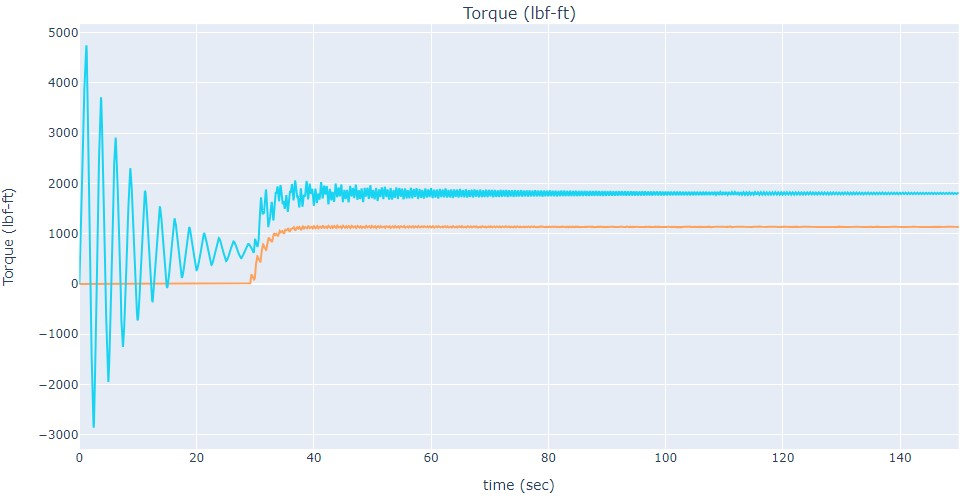
\includegraphics[width=6.5in]{Torque_onbottom}
  \caption{Torque for On bottom case}\label{torque_onbottom}
\end{figure}
\begin{figure}
  \centering
  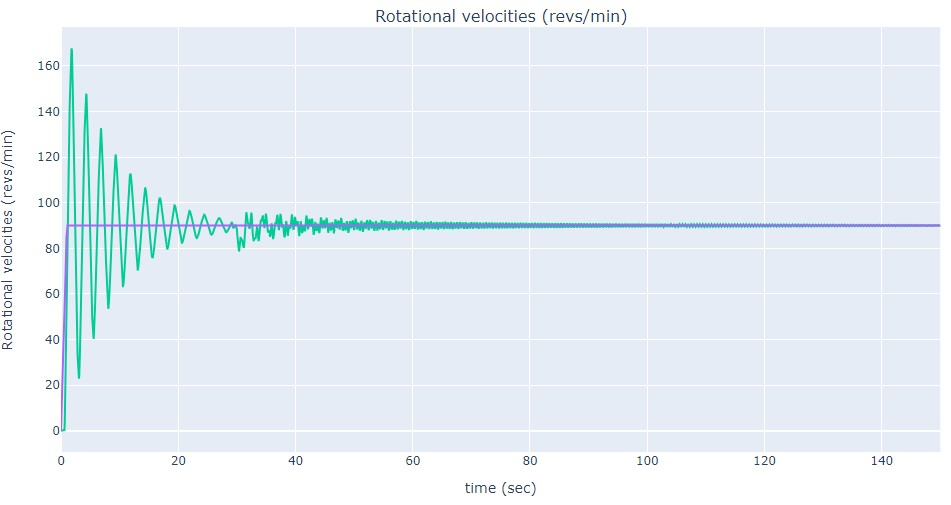
\includegraphics[width=6.5in]{RPM_onbottom}
  \caption{RPM for on bottom case}\label{RPM_onbottom}
\end{figure}
\begin{figure}
  \centering
  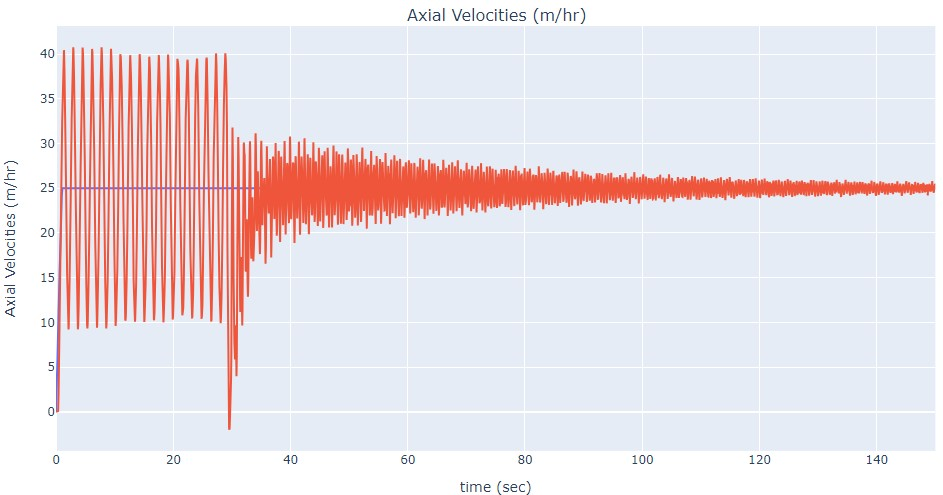
\includegraphics[width=6.5in]{bit_vel_onbottom}
  \caption{Bit velocity for on bottom case}\label{bit_vel_onbottom}
\end{figure}
\begin{figure}
  \centering
  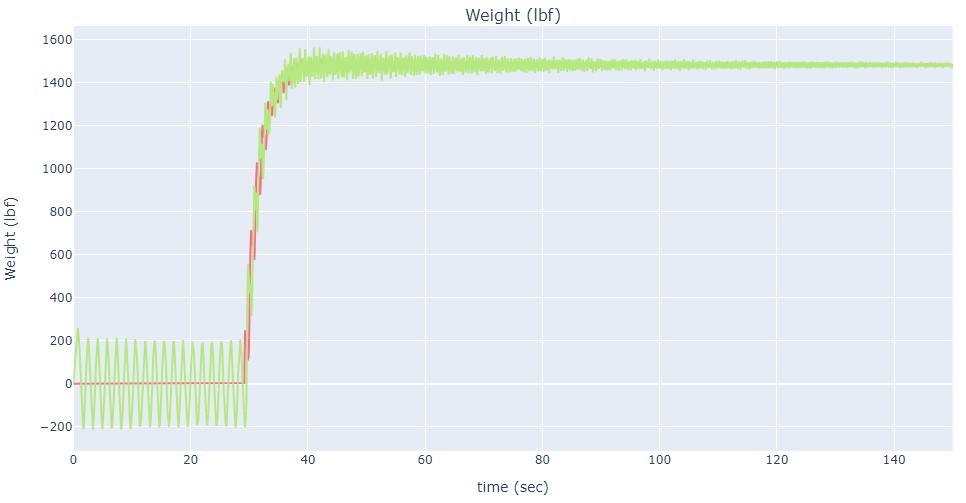
\includegraphics[width=6.5in]{wob_onbottom}
  \caption{Weight on bit for on bottom case}\label{wob_onbottom}
\end{figure}
\begin{figure}
  \centering
  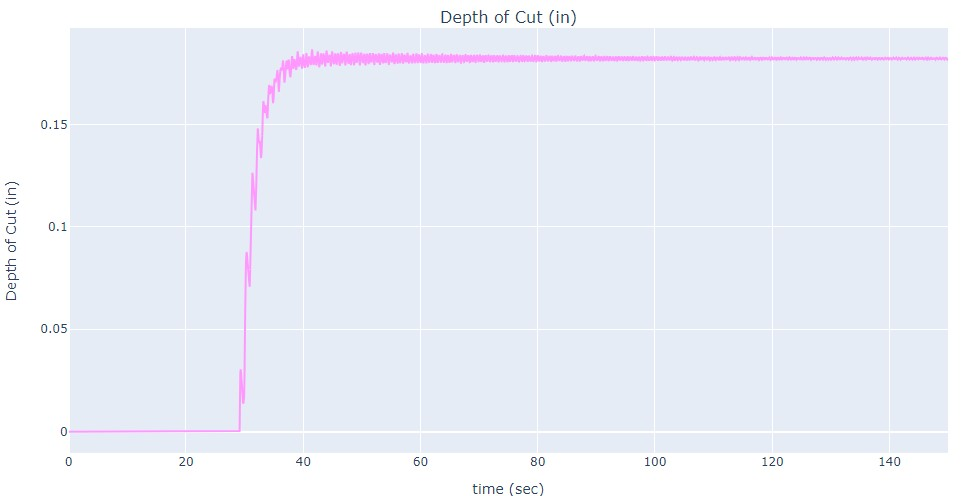
\includegraphics[width=6.5in]{DOC_onbottom}
  \caption{Depth of cut for on bottom case}\label{doc_onbottom}
\end{figure}
\begin{figure}
  \centering
  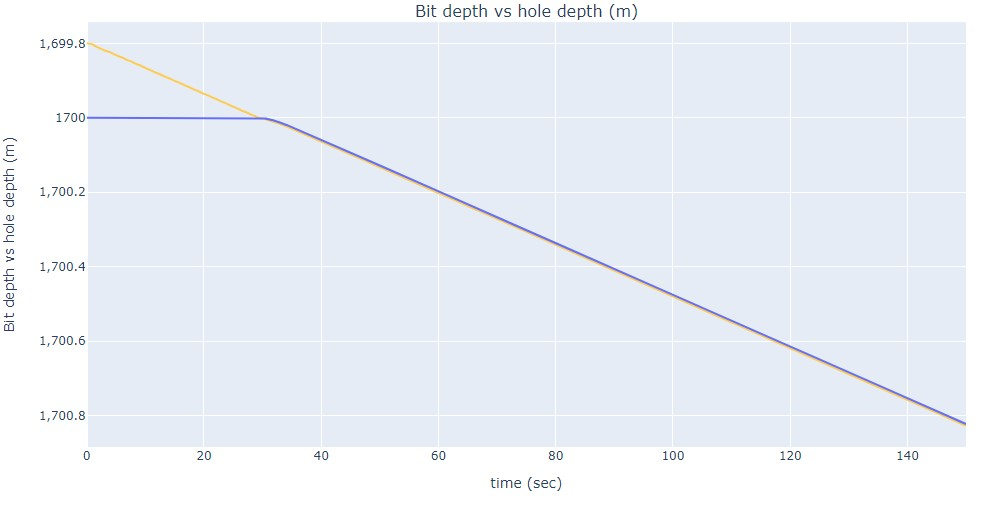
\includegraphics[width=6.5in]{depth_onbottom}
  \caption{Bit and Hole depths for on bottom case}\label{depth_onbottom}
\end{figure}

